\documentclass[tikz,border=10pt]{standalone}
\usepackage[T1]{fontenc}
\usepackage{lmodern}
\usetikzlibrary{calc}
\definecolor{ink}{HTML}{183444}
\definecolor{blue}{HTML}{1B6780}
\definecolor{amber}{HTML}{AD601A}
\begin{document}
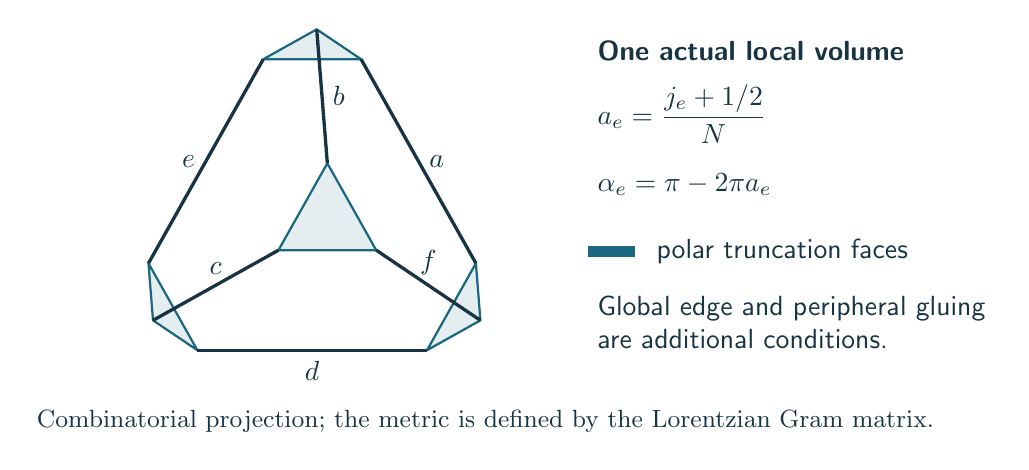
\begin{tikzpicture}[font=\sffamily,text=ink,line join=round]
 \coordinate(A)at(0,3.8);\coordinate(B)at(-2.7,-1);\coordinate(C)at(2.7,-1);\coordinate(D)at(.25,.65);
 \foreach \v/\w in {A/B,A/C,A/D,B/A,B/C,B/D,C/A,C/B,C/D,D/A,D/B,D/C}{\coordinate(\v\w)at($(\v)!.23!(\w)$);}
 \filldraw[fill=blue!12,draw=blue,line width=.8pt](AB)--(AC)--(AD)--cycle;
 \filldraw[fill=blue!12,draw=blue,line width=.8pt](BA)--(BC)--(BD)--cycle;
 \filldraw[fill=blue!12,draw=blue,line width=.8pt](CA)--(CB)--(CD)--cycle;
 \filldraw[fill=blue!12,draw=blue,line width=.8pt](DA)--(DB)--(DC)--cycle;
 \draw[ink,line width=1.2pt](AB)--node[left]{$e$}(BA);
 \draw[ink,line width=1.2pt](AC)--node[right]{$a$}(CA);
 \draw[ink,line width=1.2pt](BC)--node[below]{$d$}(CB);
 \draw[ink,line width=1.2pt](AD)--node[right]{$b$}(DA);
 \draw[ink,line width=1.2pt](BD)--node[above]{$c$}(DB);
 \draw[ink,line width=1.2pt](CD)--node[above]{$f$}(DC);
 \node[anchor=west]at(3.5,2.8){\textbf{One actual local volume}};
 \node[anchor=west]at(3.5,2){$\displaystyle a_e=\frac{j_e+1/2}{N}$};
 \node[anchor=west]at(3.5,1.1){$\alpha_e=\pi-2\pi a_e$};
 \draw[blue,line width=4pt](3.5,.25)--(4.1,.25);\node[anchor=west]at(4.25,.25){polar truncation faces};
 \node[anchor=west,text width=5cm,align=left]at(3.5,-.65){Global edge and peripheral gluing are additional conditions.};
 \node[font=\small]at(2.2,-1.9){Combinatorial projection; the metric is defined by the Lorentzian Gram matrix.};
\end{tikzpicture}
\end{document}
